\documentclass{report}
\usepackage[english]{babel}
\usepackage[utf8]{inputenc}
\usepackage[T1]{fontenc}
\usepackage{listings}
\usepackage{titlesec}
\usepackage{color}
\usepackage{graphicx}
\usepackage{geometry}
\geometry{hmargin=2.5cm,vmargin=3.5cm}

\titleformat{\chapter}[display]
            {\normalfont\bfseries}{}{0pt}{\Huge}

\lstset{ escapeinside={(*}{*)} }

\title{\textbf{Rapport IHM PROG6}\\Pingouin}

\author{Castel Antonin, Reboul Paul, Soret Louka, Sorin Gaëtan, Vandendorpe Thomas}
\begin{document}

\maketitle{}
\tableofcontents
\chapter{Introduction}
bla bla bla
\chapter{Menu}.
\section{Truc}
blabla

\section{Truc}
blabla

%pour les espaces:
%\hspace{0.5cm}
%\vspace{0.7cm}

\chapter{Scene de jeu}
\section{Plateau}
Le plateau est évidemment l'élément pincipal, c'est pourquoi c'est l'élément le plus grand et qu'il est centré. Cependant beaucoup d'intéractions sont possible avec ce plateau. Suite aux tests IHM,
nous avons constaté que les joueurs, lors de la première utilisation du jeu, comprennent mieux les éléments intéractifs si ces derniers sont dynamiques (clignotement, mouvement, ...).

\begin{itemize}
\item Poser un pingouin: mise en évidence des cases à 1 poissons lors de la phase de pose des pingouins. La couleur de la case est de la couleur du joueur courant et clignote pour signaler un objet avec lequel on peut interragir.
  \begin{center}
    
    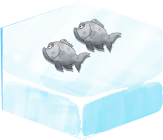
\includegraphics[width=2cm]{image/bloc_simple.png}    
    \hspace{1cm}
    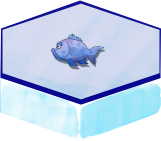
\includegraphics[width=2cm]{image/bloc_mev.png}
    \\
    bloc non cliquable \hspace{0.5cm} bloc cliquable
  \end{center}

\item Selectionner un pingouin: les pingouins sont tous identifiés par des ronds de la couleur de son joueur en dessous de lui. Nous avons ensuite rajouté une flèche sur les pingouins déplaçable du joueur courant. Ces flèches bouge indiquant qu'on peut intéragir avec le pingouin.
  \begin{center}
    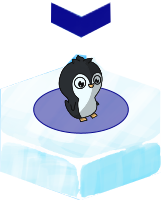
\includegraphics[width=2cm]{image/bloc_pingouin.png}    
  \end{center}
\end{itemize}


\end{document}
